\section{Case Study: Spacecraft Rendezvous Passive Safety}
\label{sec:casestudy}

We evaluate our method on a spacecraft rendezvous passive safety case study. The system consists of a primary chaser spacecraft moving towards a secondary, free-flying object (such as a satellite) and performing close-proximity maneuvers.
%
The maneuver is analyzed in relative coordinates, as shown in Figure~\ref{fig:chaser}.
%
The verification goal is to ensure \emph{passive safety}: at any time in the maneuver, a system failure may occur and the resulting propulsion-free trajectory must avoid colliding with the target satellite.
%
This requirement comes from real-world failures. In 2005, NASA’s DART spacecraft was intended to rendezvous with the MUBLCOM satellite, but due to depleted propellant instead collided with the target satellite (a loss of a
\$110 million project)~\cite{croomes2006overview}.

\begin{figure}[t]
\centerline{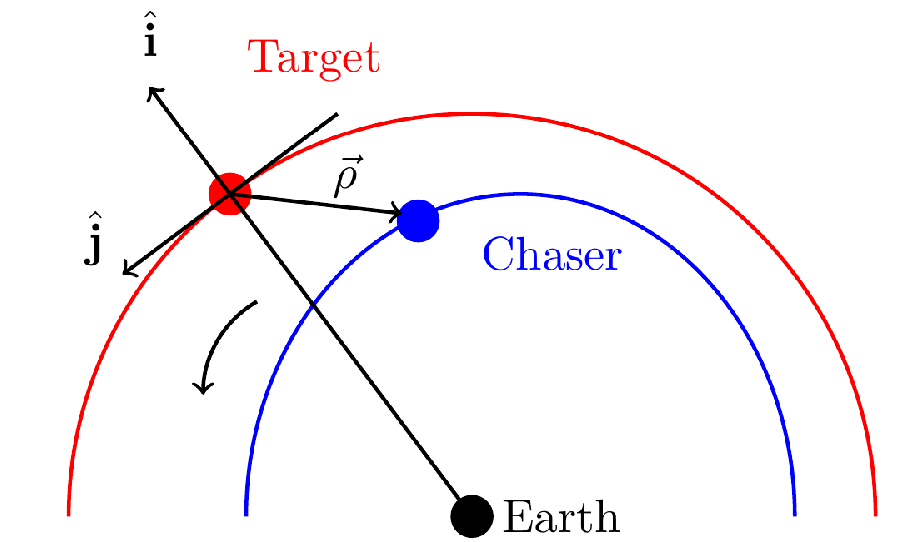
\includegraphics[width=0.5\columnwidth]{images/chaser.png}}
\caption{Collisions are checked between spacecraft in orbit in relative coordinates (image from~\cite{chan2017verifying}).}
\label{fig:chaser}
\end{figure}

Our model is based on a published benchmark for this system~\cite{chan2017verifying,jewison2016spacecraft}. The system is modeled as a hybrid automaton with different discrete modes depending on the sensors being used for navigation, and an LQR controller is designed to meet physical and geometric safety constraints.
%
The relative dynamics are linearized using the Clohessy-Wiltshire-Hill (CWH) equations~\cite{wh1960terminal}, which is often used in close proximity operations. The hybrid automaton consists of three modes, two for different navigation strategies, and one for the passive dynamics, shown in Figure~\ref{fig:ha}.
%
In our analysis, we check for passive safety over the full time bound, $t1=0$ and $t_2=200$.
%
We focus on the collision-free safety property that the spacecraft must remain 0.2 meters apart at all times.

\begin{figure}[t]
\centerline{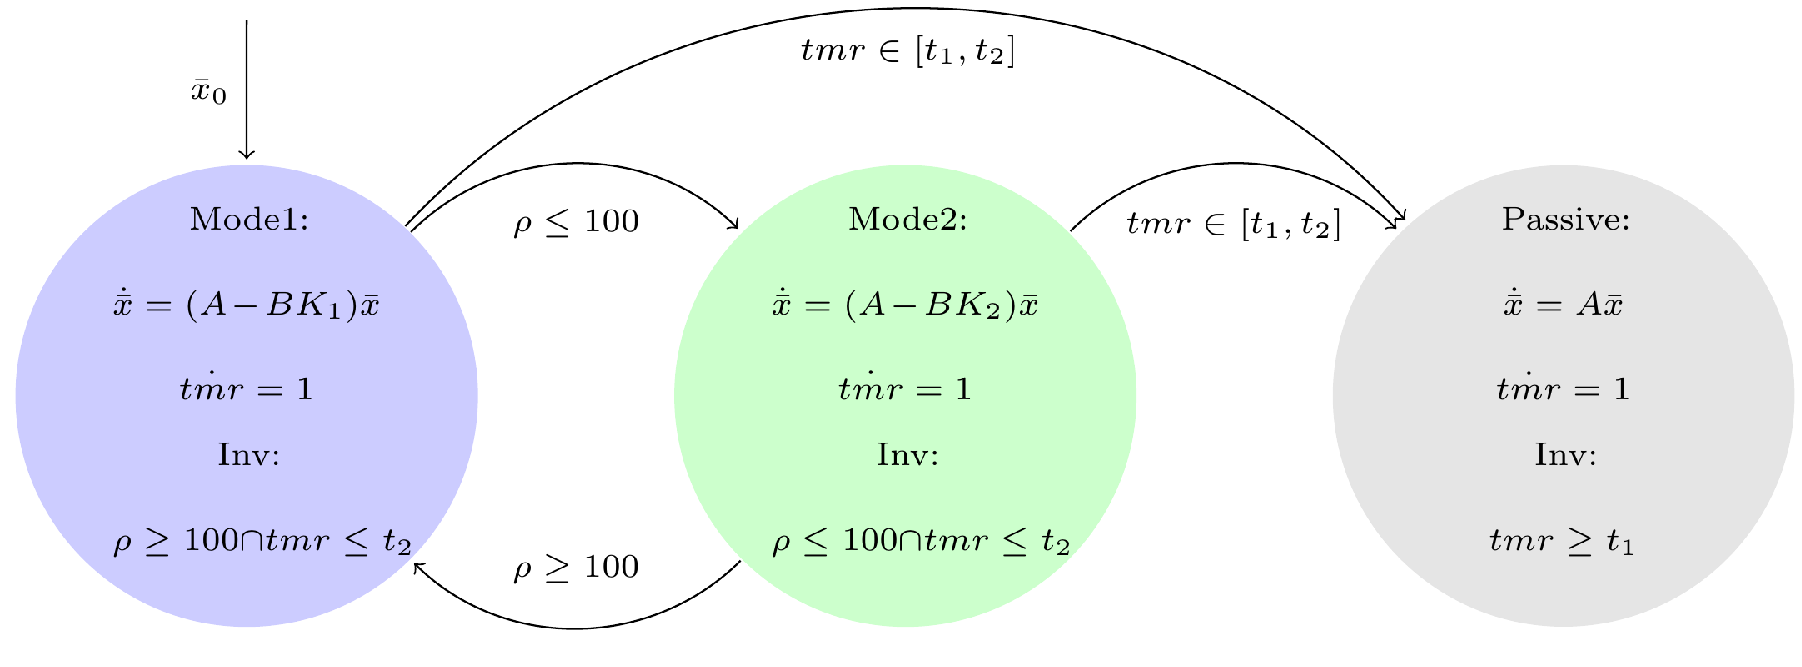
\includegraphics[width=0.9\columnwidth]{images/ha.png}}
\caption{Hybrid automaton model of case study (image from~\cite{chan2017verifying}). We check for passive safety over the full time bound ($t_1=0$ and $t_2=200$).}
\label{fig:ha}
\end{figure}

Although several tools have successfully analyzed a version of this model in the ARCH hybrid systems tools competition in 2018~\cite{archcomp18linear}, a critical simplification was made: the competition model did not actually check the passive safety requirement. In particular, the competition model used a \emph{fixed} time to transition to the passive model. This is an unrealistic simplification, since the time of failure cannot not be known in advance. 

The analysis done in the original work~\cite{chan2017verifying} is slightly better, in that it checks for passive safety for a known 5 minute failure interval during the 200 minute maneuver. The reason stated in the paper for this is that, if larger time intervals are used,
``the initial set of states under the Passive mode is large, making it very difficult to prove safety.'' The suggestion is then to create subintervals that cover the full time range of transitions to the passive mode, and then run several experiments. Presumably, a manual guess-and-check approach should be used to create these subintervals.

The full passive safety problem can be solved using the proposed aggdag method. Our aggdag method performs full state aggregation (an overapproximation), and then recursively desegregates if the overapproximation reaches an error mode. The advantage of this is that (1) the method is fully automatic, (2) steps where the overapproximation is safe can be skipped by the refined sets, which is more efficient than using multiple independent experiments, and (3) if an error exists, it will be detected after full deaggregation is performed, which allows the generation of a concrete counter example trace. Other verification tools for linear hybrid systems do not typically generate counter-examples when safety cannot be proven.

Our experiments are performed on a system with an Intel i5-5300U CPU running at 2.30GHz with 16GB RAM and using Ubuntu Linux 18.04.
%
We first analyze the runtime of the method, shown in Table~\ref{tab:runtime}.
%
We look at the number of seconds and the number of reachability steps needed to prove safety for the system as we vary the step size.
%
A reachability step is a single continuous post operator, or a refinement step when performing deaggregation.
%
As the step size for this system is reduced, the number of combinations of steps that reach each guard in the hybrid automaton increases.
%
However, from the table, we observe that the runtime and number of steps remains inversely proportional to the step size.
%
This means that the analysis is successfully using state set aggregation to eliminate combinatorial explosion, with sufficient
precision to guarantee the system avoid collisions.

\setlength{\tabcolsep}{2pt}
\begin{table}[t]
\caption{Safe maneuver check time.}
\label{tab:runtime}
\centering
\setlength{\aboverulesep}{0.0pt}
\setlength{\belowrulesep}{0.0pt}
\setlength{\extrarowheight}{-0.2ex}
\begin{tabular}{@{}lll@{}}
  \toprule
  Step Size & Runtime & Num Steps \\
  \midrule
  1.0 & 5.1 & 726 \\
  0.5 & 11.0 & 1508 \\
  0.2 & 34.7 & 4657 \\
  0.1 & 73.2 & 9557 \\
\bottomrule
\end{tabular}
\end{table}

The analysis is exact, in that if the system were to have a collision, the deaggregation approach would eventually find it.
%
In the next experiment, we increase the collision distance from 0.2 to 1.0 meters.
%
In this case, a collision is possible, and our approach generates the corresponding counter-example trace (initial state and switching times)
for every step size analyzed.
%
The results are shown in Table~\ref{tab:runtime_unsafe}.
%
The runtime increases compared with the safe version of the benchmark, as more deaggregation is necessary in this case since a real error trace is
present (the deaggregation continues until single time instants are considered, at which point a concrete trace can be generated).

\setlength{\tabcolsep}{2pt}
\begin{table}[t]
\caption{Unsafe maneuver check time.}
\label{tab:runtime_unsafe}
\centering
\setlength{\aboverulesep}{0.0pt}
\setlength{\belowrulesep}{0.0pt}
\setlength{\extrarowheight}{.0ex}
\begin{tabular}{@{}lll@{}}
  \toprule
  Step Size & Runtime & Num Steps \\
  \midrule
  1.0 & 9.2 & 1232 \\
  0.5 & 34.8 & 3736 \\
  0.2 & 94.7 & 10958 \\
  0.1 & 243 & 25091 \\
\bottomrule
\end{tabular}
\end{table}

Overall, our main evaluation result is that analysis of this system is possible though maintaining the aggdag data structure  and
performing deaggregation upon reaching an error mode.
%
Prior to this, all analysis on this model checked for switching to the passive mode at a single time instant or small time window, since otherwise the methods would have too much error to prove the system is safe.
%
For this reason, we could not perform a tool runtime comparison; analysis is not possible on this model with existing tools.
%
Furthermore, we were able to generate counterexamples in the cases where the safety property was violated.
